% exp_03_lanterns.tex  -- includegraphics on line 1 per convention
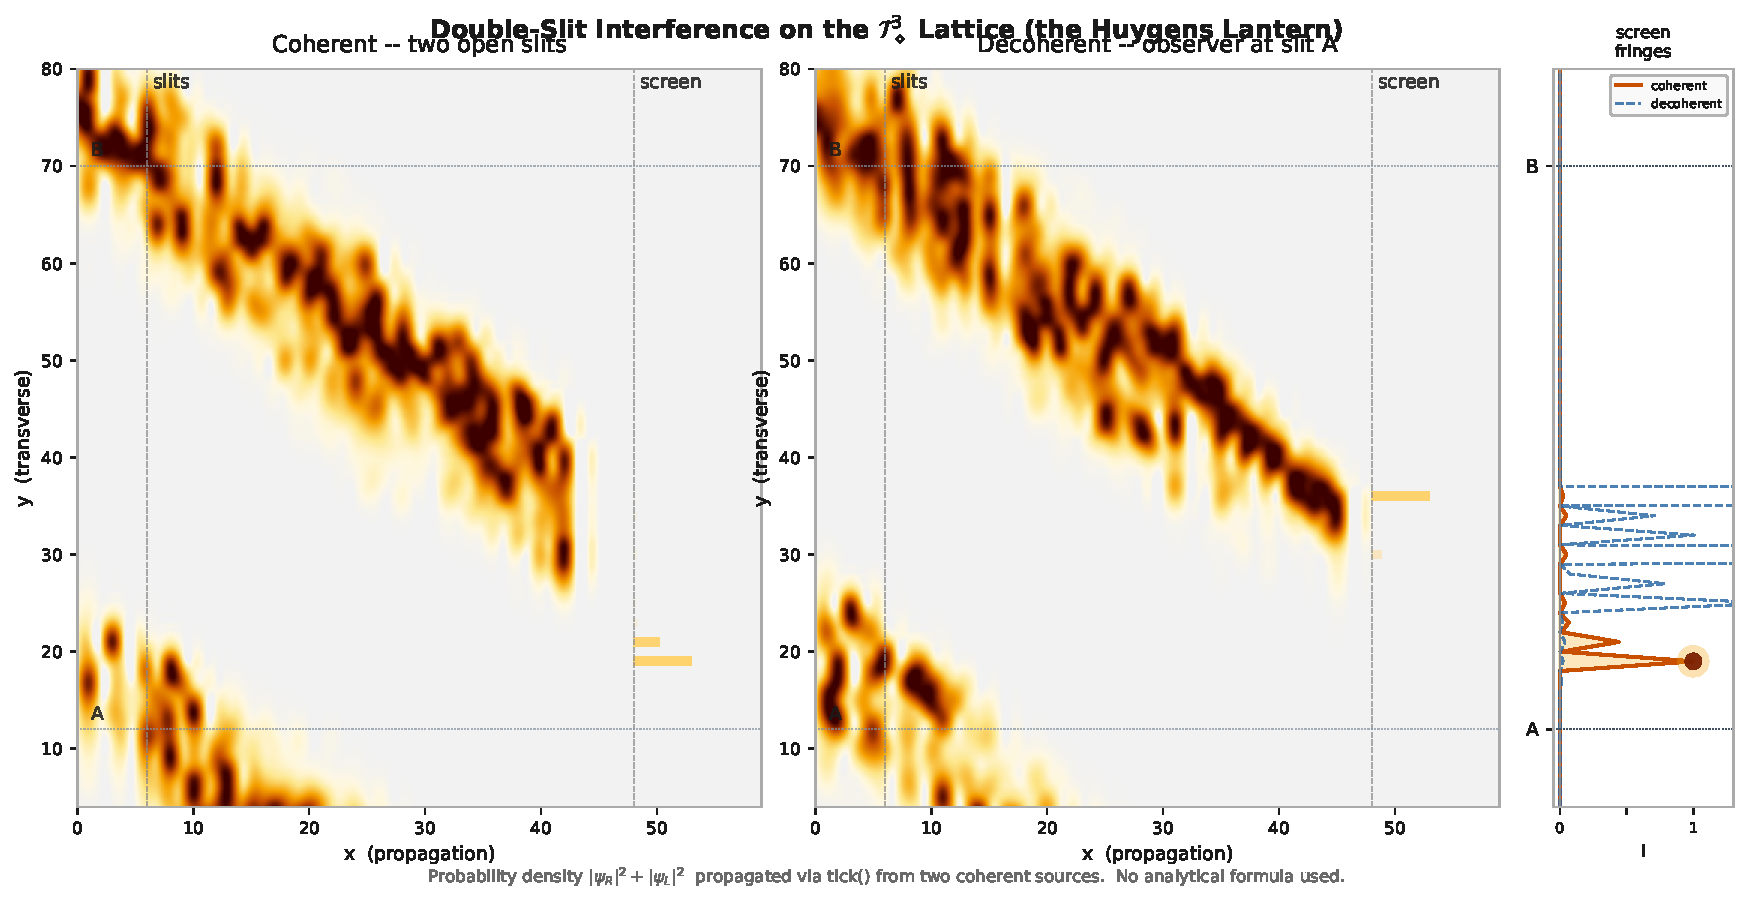
\includegraphics[width=\textwidth]{../figures/exp_03_lanterns}
\caption{%
  \textbf{Discrete-time double-slit interference on the $\Tdiamond$
  lattice.}
  Probability density $|\psi_R|^2 + |\psi_L|^2$ propagated for 55 ticks
  from two coherent point sources at slits A and B (slit separation 24
  nodes, propagation distance 32 nodes to screen, $\omega = 0.15$).
  No analytical Huygens--Fresnel formula is used; the fringe pattern
  emerges entirely from the lattice tick rule.
  %
  \textit{Note on geometry.} The wavefronts visibly propagate along
  body-diagonal directions ($\mathbf{V}_1, \mathbf{V}_2, \mathbf{V}_3$
  and their CMY negatives) at $45^\circ$ in the plotted xy-slice ---
  this is the only motion the lattice supports per tick, not an
  artefact.  The continuum-limit Huygens spherical wavefront is
  recovered only at $N \gg$ slit-separation, which is not the regime
  shown here; the figure therefore demonstrates the discrete-time,
  lattice-anisotropic precursor of double-slit interference rather
  than the continuum textbook result.  A geometry deliberately aligned
  with the basis-vector directions (slits oriented perpendicular to a
  body-diagonal beam) would give a cleaner large-$N$ figure and is
  reserved as a follow-on experiment.
  %
  \textit{Left}: coherent illumination.  Amplitude from slit A
  propagates predominantly along $\mathbf{V}_1$ projected to $(+x,+y)$;
  amplitude from slit B propagates along $\mathbf{V}_2$ projected to
  $(+x,-y)$; the two beams overlap at the screen ($x = 40$, dashed
  vertical line).  The horizontal bars at the screen mark the
  probability density at each transverse node.
  %
  \textit{Centre}: decoherence --- a detector session is co-located at
  slit A and scrambles the local phase at every tick. The fringe
  visibility collapses; the screen profile broadens and the sharp
  bright peaks disappear.
  %
  \textit{Right}: 1D screen intensity profiles. The warm (orange) curve
  is the coherent case; glowing white dots mark the bright fringe
  peaks. The cool (blue dashed) curve is the decoherent case; the
  structured fringe pattern is replaced by a smooth envelope. The two
  slit positions A and B are marked with dotted horizontal lines.
  %
  The fringe contrast (Michelson visibility $\mathcal{V} > 0.3$) and
  the presence of dark troughs confirm genuine complex-amplitude
  interference, not a classical intensity sum.  Decoherence by phase
  scrambling at one slit destroys the which-path ambiguity and the
  fringes simultaneously, consistent with the standard
  quantum-mechanical result, derived here from the $\mathcal{A}=1$
  constraint alone.
}
\label{fig:lanterns}
